\documentclass[english]{article}
\usepackage{amsmath}
\usepackage[letterpaper]{geometry}
\usepackage[table,xcdraw]{xcolor}
\usepackage{gensymb}
\usepackage{graphicx}
\graphicspath{ {images/} }
\geometry{verbose,tmargin=1in,bmargin=1in,lmargin=1in,rmargin=1in}
\newcommand\numberthis{\addtocounter{equation}{1}\tag{\theequation}}

\title{ESE 650 Project 4 report: Simultaneous localization and mapping (SLAM) using particle filters }
\author{Dhruva Kumar}
\date{}

\begin{document}

\maketitle

\section{Introduction}
This project aims to simultaneously localize and map a robot in an unknown indoor environment using odometry data, IMU, and a lidar scanner. A particle filter based approach is taken to achieve the objective. Particle filters effectively model a probability distribution (dynamic model) as a set of discrete states. Each particle has an associated weight which describes its confidence in its current estimate according to the observation. The THOR robot is used for this project.  

\section{SLAM}
\begin{itemize}
\item A log odds grid map is used to map the bot and update its values (occupied cells and free cells) based on the lidar scan hits. A 1500 x 1500 map is used with a grid resolution of 5cm per cell.
\item The head pitch, neck yaw and torso yaw are taken into consideration. 
\item Initially, 100 particles are taken and are initialized with position (0,0) and the orientation is randomized according to a normal distribution with a variance of 20\degree. The log odds grid map is updated with the lidar scans of the first iteration. The particle weights are initialized to one. 
\item \textbf{Dynamic update}: Subsequently for each iteration, the motion of all the particles are updated according to the odometry data:
\begin{align*}
	\begin{bmatrix}
	x_{i}^{t} \\ y_{i}^{t}
	\end{bmatrix} =&\; 
	\begin{bmatrix}
	x_{i}^{t-1} \\ y_{i}^{t-1}
	\end{bmatrix} + 
	\begin{bmatrix}
	\cos\alpha & -\sin\alpha \\
	\sin\alpha & \cos\alpha
	\end{bmatrix}
	\begin{bmatrix}
	dx \\ dy
	\end{bmatrix} + 
	\begin{bmatrix}
	\mathcal{N}(0,\sigma_x) \\ \mathcal{N}(0,\sigma_y)
	\end{bmatrix} \numberthis \\
	\theta_{i}^{t} =&\; \theta_{i}^{t-1} + d\phi \numberthis \\
  	 \text{where, } d\phi =&\; \phi_{i} - \phi_{i-1} \\
  	\alpha =&\; \theta_{i-1} - \phi_{i-1}
\end{align*}
$(x,y,\theta)$ is the pose for each particle $i$ for the $t^{th}$ iteration. $\phi$ is the yaw of the bot derived from integrating the gyroscope of the IMU. \\
Equation (1) and (2) is the motion model for the particles. The position of each particle is updated by its previous position + the difference in x and y from the odometry data rotated by $\alpha$. Here, $\alpha$ is the difference between the previous orientation of the bot and previous bot yaw. Gaussian noise with a variance of $\sigma$ is also added to the position of each particle. The orientation $\theta$ of each particle is updated by the difference in the yaw procured from the odometry data. $\sigma_x$ and $\sigma_y$ are kept as 0.3. The variance induced in the position of the particles mattered significantly in performance. The higher the value, the better the performance. However, it shouldn't be set too high for all the particles to diverge. \\

\item \textbf{Weight update}: The weights of the particles are updated and resampled if required.
\begin{itemize}
	\item The weights of the particles are set based on the lidar hits according to the pose for each particle. The particle whose map corresponds highly to the previous log odds map is given more weight. In this case, the weights are calculated by summing up over the lidar hits or occupied cells by a factor of 0.02. This worked pretty well. The current weight vector is multipled by its previous weight which is used as a prior here to use the previous information. This is then normalized to sum upto 1. 
	\item Before computing the weights, the lidar scans neglected for invalid ranges. This is done for scan $<$ 0.3, scan $>$ 30 and for pitch correction. The lower limit 0.3 should be as low as possible to account for all the hits. However, it should also account for instances of gantry hits. 0.3 seemed to work well in general. If the head pitch is above a threshold, scans at the sides (0\degree $\pm$ thresh-angle and 180\degree $\pm$ thresh-angle) are retained, while the rest is removed. Ranges from 35 to 55 \degree worked well for thresh-angle. The threshold for the head pitch was computed based on:
	\begin{align*}
	scan_{center} > \frac{r}{\sin \gamma}
	\end{align*}
	Here, $scan_{center}$ refers to the lidar scan of the forward position where the bot is looking at. r refers to the diagonal of the right angled triangle if the height of the triangle is the height of the bot. $\gamma$ refers to the head pitch. 
	The above formulation worked well for the train set. However, a hard thresholding of pitch > 0.25 radians worked better and this was used. 
	
	\item Resampling is done if the following condition is satisfied:
	\begin{align*}
	N_{effective} =&\; \frac{(\sum_{i=1}^N w_i )^2}{\sum_{i=1}^{N} w_i^2} < threshold 
	\end{align*}
	The threshold was kept as 0.2. When resampled, the weight vector is set to ones. This threshold should be less. If it's too large, resampling is done really frequently and at any given time, there will be a few set of particles in the cluster.  
	\item The chosen bot position is the particle with the highest weight. 
\end{itemize}

\item \textbf{log odds map update}: The log odds map is updated with the lidar scans of the best particle chosen.
\begin{itemize}
	\item The occupied cells are incremented by $10 \log r$. $\log r$ was kept as 0.02. 
	\item The free cells in the map were decremeted by $\log r$. 
	\item The values of the log map were limited to 3 to prevent certainty. This threshold mattered significantly in the performance of SLAM. 
\end{itemize}


\end{itemize}

\section {Results}

The loop closure for the test set doesn't happen perfectly. But it's still pretty decent nonetheless. The performance on the train data is pretty good. 

\begin{figure}[h]
\centering
\includegraphics[scale=0.65]{slam_test_result}
\caption{Test set with path}
\end{figure}

\begin{figure}[h]
\centering
\includegraphics[scale=0.65]{slam_test_result1}
\caption{Test set}
\end{figure}


\begin{figure}[h]
\centering
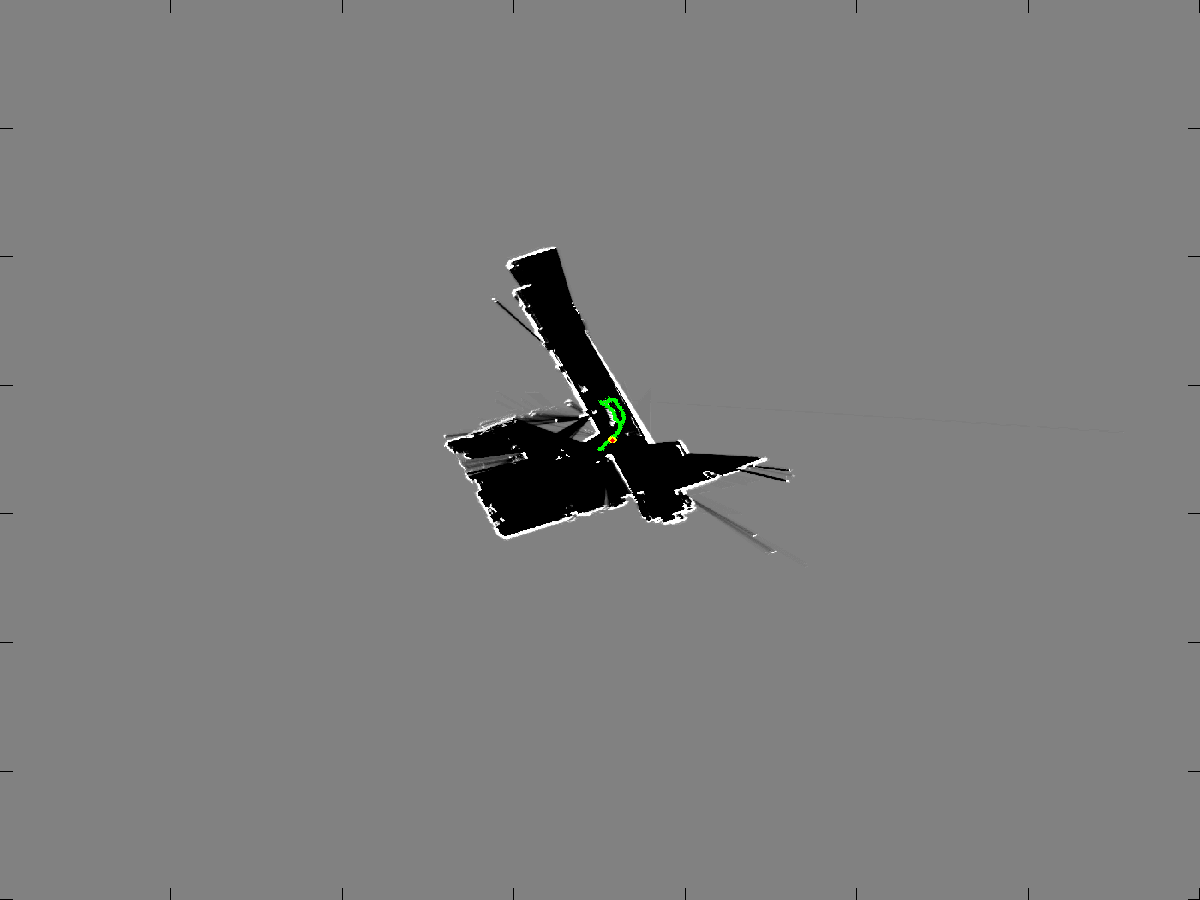
\includegraphics[scale=0.65]{slam0_result}
\caption{Dataset 0 with path}
\end{figure}

\begin{figure}[h]
\centering
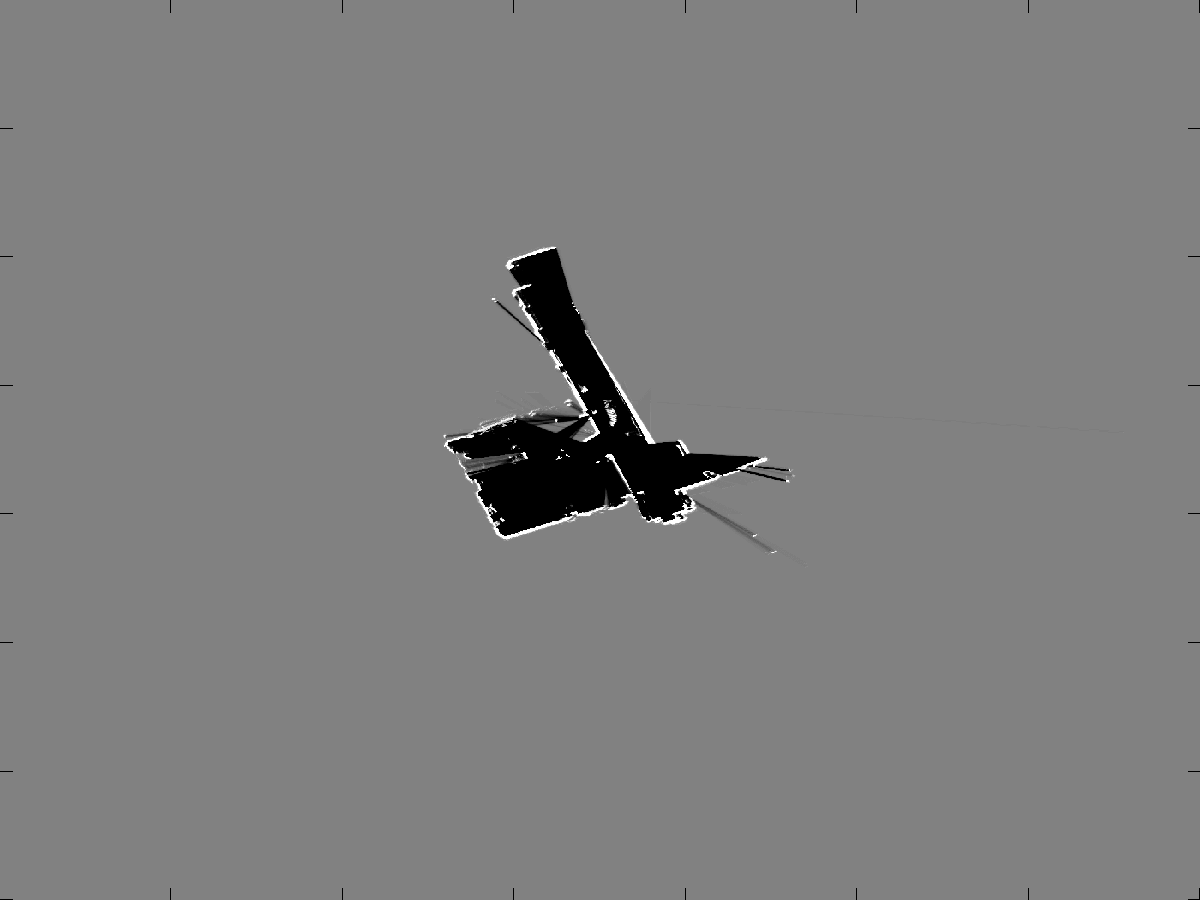
\includegraphics[scale=0.65]{slam0_result1}
\caption{Dataset 0}
\end{figure}

\begin{figure}[h]
\centering
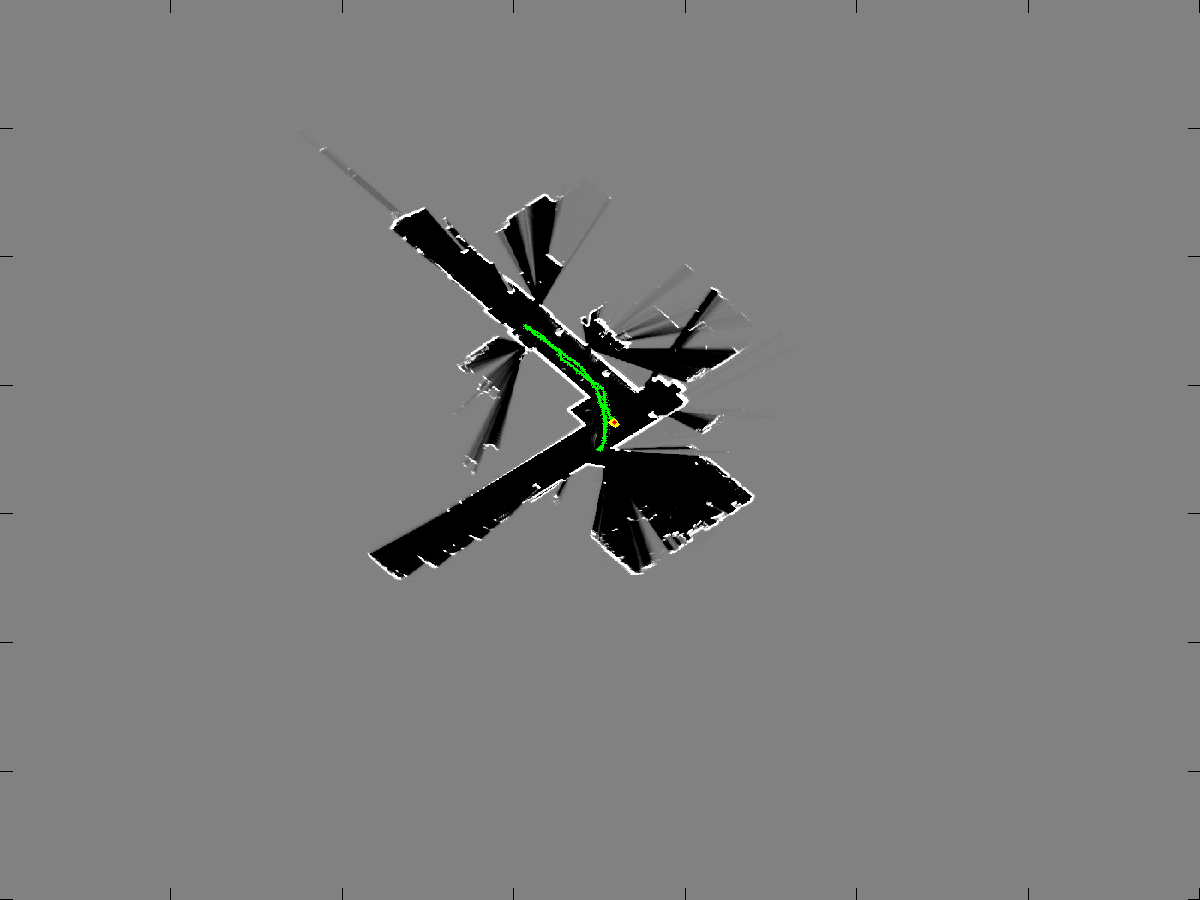
\includegraphics[scale=0.65]{slam2_result}
\caption{Dataset 2 with path}
\end{figure}

\begin{figure}[h]
\centering
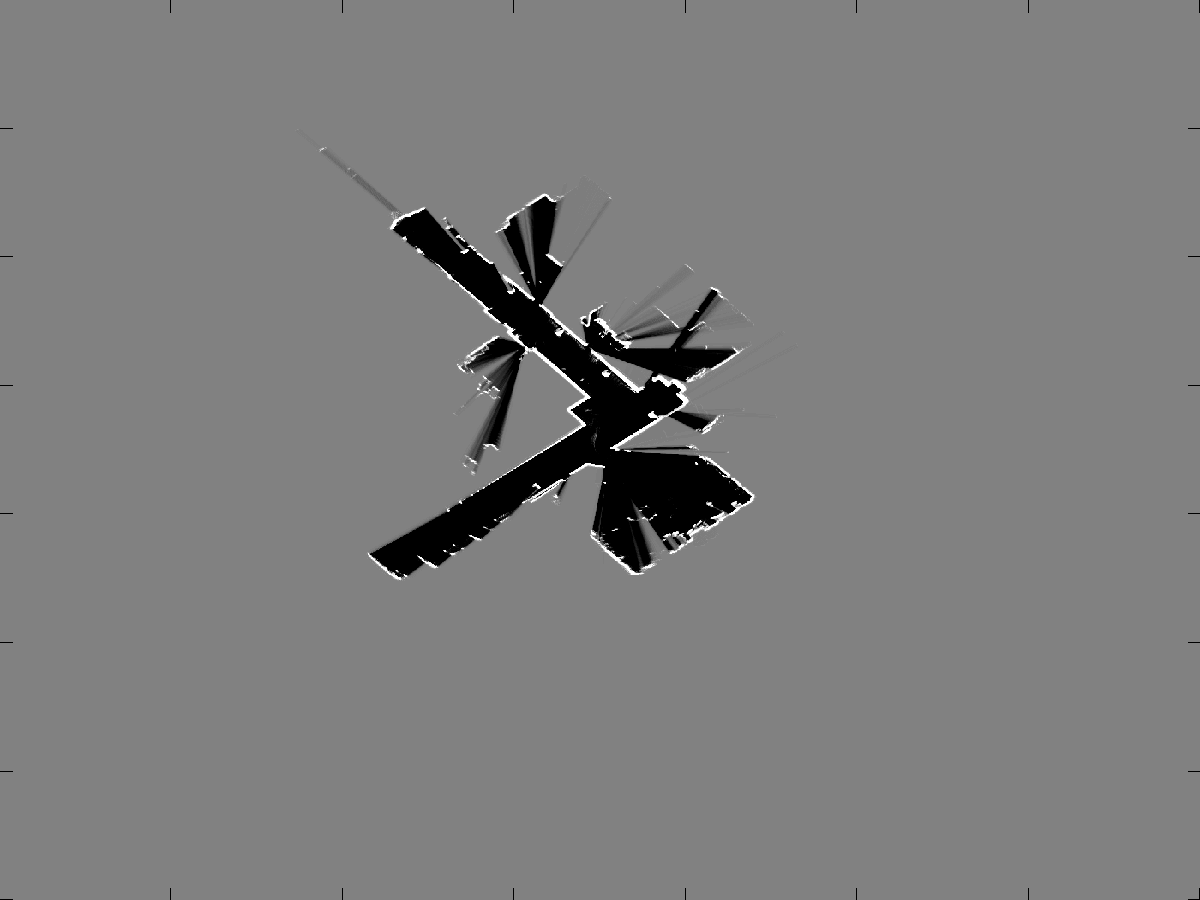
\includegraphics[scale=0.65]{slam2_result1}
\caption{Dataset 2}
\end{figure}

\begin{figure}[h]
\centering
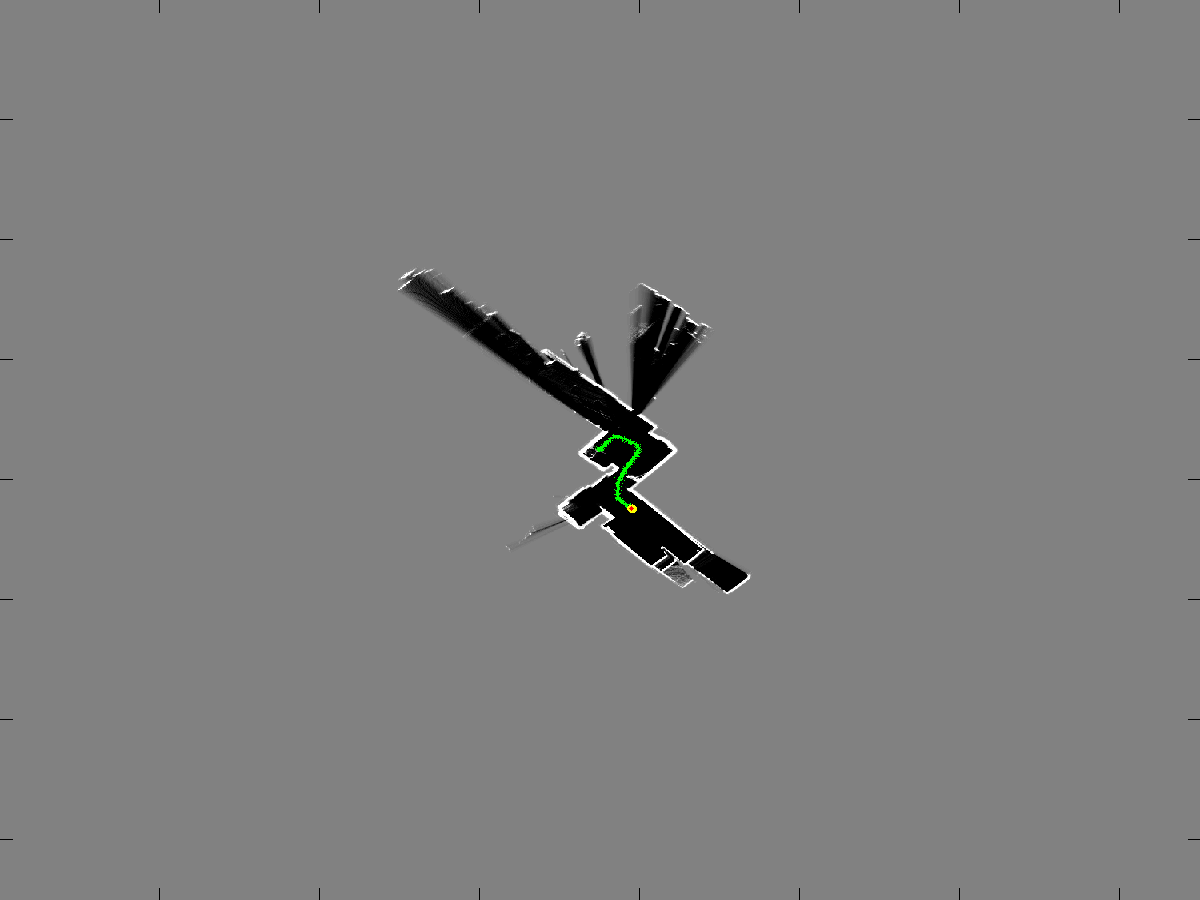
\includegraphics[scale=0.65]{slam3_result}
\caption{Dataset 3 with path}
\end{figure}

\begin{figure}[h]
\centering
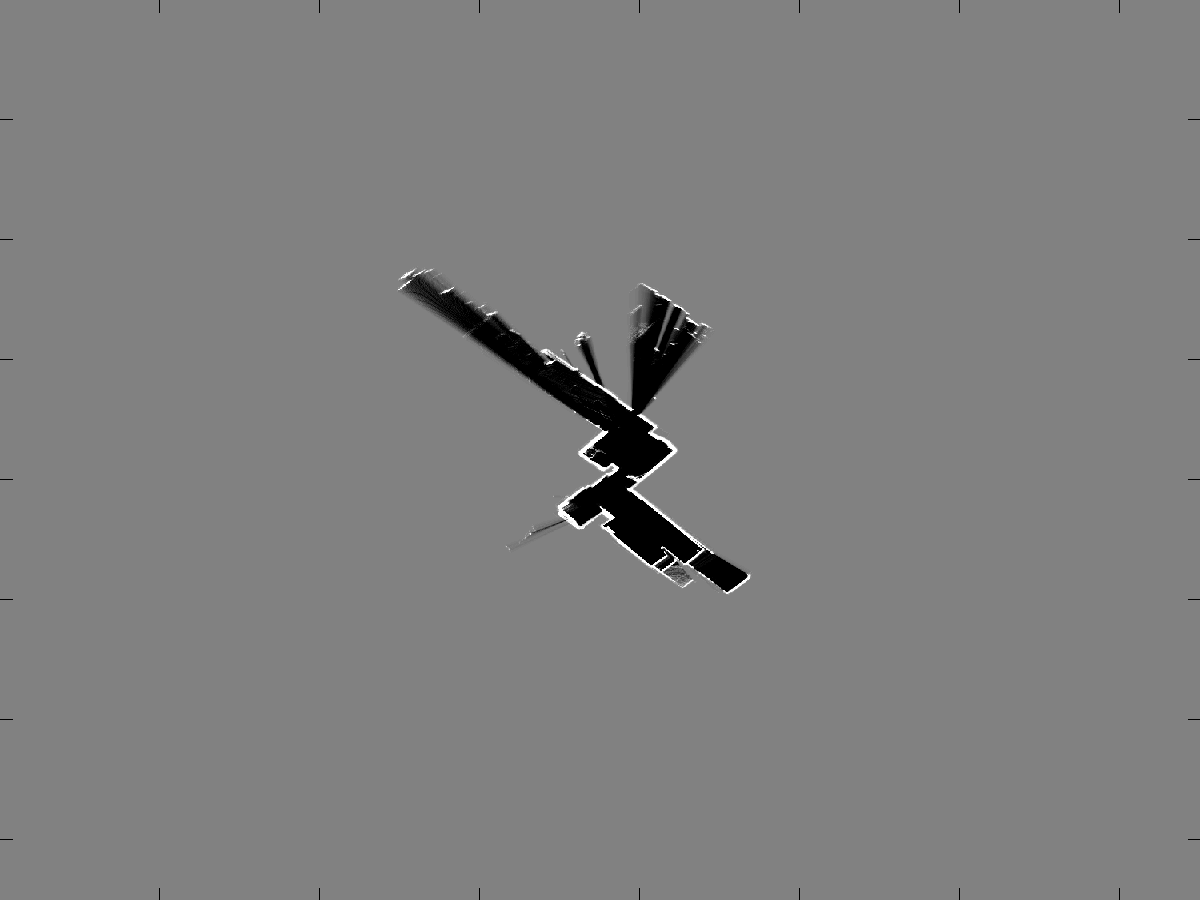
\includegraphics[scale=0.65]{slam3_result1}
\caption{Dataset 3}
\end{figure}

%Initially, the partices are assigned In the prediction/expection phase, the particles are updated via the dynamic model according to the odometry data. In the measurement update phase, 

\begin{thebibliography}{99}
\bibitem{c1} Dr. Daniel Lee ESE 650 lecture notes. 
\end{thebibliography}

\end{document}
